\documentclass{beamer}
\usetheme[secheader]{Madrid}
\usecolortheme{dolphin}
\setbeamertemplate{navigation symbols}{}

\usepackage{graphicx}
\usepackage{fontawesome}
\usepackage{multicol}

\newcommand{\highlight}[1]{{\color{red} #1}}

\titlegraphic{
    \begin{minipage}{0.49\textwidth}
        \centering
        
\includegraphics[height=0.2\textwidth]{assets/logo_ciemat}
    \end{minipage}
    \begin{minipage}{0.49\textwidth}
        \centering
        
\includegraphics[height=0.2\textwidth]{assets/logo_euramet}
        
\includegraphics[height=0.2\textwidth]{assets/logo_tc_ir}
    \end{minipage}
}

\title[TC IR: Digital Transformation]{Digital Transformation}
\subtitle[EURAMET TC IR]{EURAMET Technical Committee for Ionising Radiation\\Annual Contact Person Meeting}
\date[1-3 April 2025]{1\textsuperscript{st} to 3\textsuperscript{rd} of April, 2025}
\author[X. Campo]{Xandra Campo}
\institute[CIEMAT]{CIEMAT, Spain}

\begin{document}

    \maketitle

    \logo{
        \vspace*{10cm}
%        
\includegraphics[height=1cm]{assets/logo_euramet}
%        
\includegraphics[height=1cm]{assets/logo_tc_ir}
        
\includegraphics[height=1cm]{assets/logo_ciemat}
    }

    \begin{frame}
        \frametitle{Table of Contents}
        \tableofcontents[hideallsubsections]
    \end{frame}


    \section{Metrology organizations for digital transformation}

    \begin{frame}
        \frametitle{Metrology organizations for digital transformation}
        %\framesubtitle{Lorem ipsum}
        Metrology organizations related with digital transformation
        \begin{itemize}
            \item CIPM:
            \begin{itemize}
                \item \textbf{CCRI-DT-TG}: Consultative Committee for Ionizing Radiation, Task Group on Digital Transformation
                    {\color{blue} \href{https://www.bipm.org/en/committees/cc/ccri/wg/ccri-dt-tg}{\faExternalLink}}
            \end{itemize}
            \item EURAMET:
            \begin{itemize}
                \item \textbf{TC-IM WG M4D}: Technical Committee for Interdisciplinary Metrology: Working Group on Metrology for Digital Transformation
                    {\color{blue} \href{https://www.euramet.org/technical-committees/tc-im/metrology-for-digital-transformation}{\faExternalLink}}
                \item \textbf{EMN Mathmet}: European Metrology Network for Mathematics and Statistics
                    {\color{blue} \href{https://www.euramet.org/european-metrology-networks/mathmet}{\faExternalLink}}
            \end{itemize}
        \end{itemize}
    \end{frame}

    \subsection{CIPM CCRI-DT-TG}

    \begin{frame}
%        \frametitle{Metrology organizations for digital transformation}
%        \framesubtitle{CCRI Task Group on Digital Transformation}
        \frametitle{CCRI Task Group on Digital Transformation}
        Goals:
        \begin{itemize}
            \item \textbf{Advise the CCRI} on the SI Digital Framework and the implications of the digital transformation for ionising radiation metrology
            \item \textbf{Act as a forum} to exchange information on progress and to create synergies and opportunities for collaboration in this field
        \end{itemize}
        Short-term priorities:
        \begin{itemize}
            \item Kind of \textbf{quantities identification} in view of the digitalisation of service categories of the KCDB
            \item Discuss how “\textbf{digital traceability chain}” could be implemented for applications in the three sections
            \item Collect use cases and user needs from the three sections
        \end{itemize}
    \end{frame}

    \subsection{EURAMET TC-IM WG M4D}

    \begin{frame}
%        \frametitle{Metrology organizations for digital transformation}
%        \framesubtitle{TC-IM WG on Metrology for Digital Transformation}
        \frametitle{TC-IM WG Metrology for Digital Transformation}
        Goals:
        \begin{itemize}
            \item \textbf{Bring together the expertise} of EURAMET members in data management, digital certificates and processes, Internet of Things and sensor networks
            \item Support EURAMET in implementing a \textbf{strategic digital transformation} aligned with the aims of the EC and EURAMET members
        \end{itemize}
        Areas of activity:
        \begin{itemize}
            \item Research \textbf{data management} according to the FAIR principles and its relation to the European Open Science Cloud
            \item \textbf{Digital certificates for calibration}, testing and conformity assessment
            \item Metrology for \textbf{internet of things} and \textbf{sensor networks}
        \end{itemize}
    \end{frame}

    \subsection{EURAMET EMN Mathmet}

    \begin{frame}
%        \frametitle{Metrology organizations for digital transformation}
%        \framesubtitle{EMN for Mathematics and Statistics}
        \frametitle{EMN for Mathematics and Statistics}
        Goals:
        \begin{itemize}
            \item \textbf{Integration} between measurement science and mathematical and statistical methods
            \item Fostering mathematical and statistical \textbf{applications} for metrology
            \item \textbf{Best practices} in mathematics and statistics in metrology
        \end{itemize}
        Areas of activity:
        \begin{itemize}
            \item \textbf{Modelling \& simulation}: Accurate modeling measurement processes and assessment of uncertainties
            \item \textbf{Data analysis \& uncertainty}: How to model data and calculate uncertainty for complex measurement processes
            \item \textbf{Artificial intelligence}: How can AI improve metrology \& vice versa
            \item \textbf{Quality assurance tools}: Research outputs in the form of data, software and guidelines consistent with the aims of NMIs and DIs
        \end{itemize}
    \end{frame}


    \section{EURAMET strategy on metrology for digital transformation}

    \begin{frame}
        \frametitle{EURAMET strategy on digital transformation}
%        \framesubtitle{Goal and status}
        \textbf{Goal}: support the digital transformation of industry and society, aligning with the EC's 2020 strategy ``Shaping Europe's digital future''.
        \bigskip

        Current status:
        \begin{enumerate}
            \item \textbf{Digitalisation efforts}: European NMIs are actively involved in digitalisation through numerous research projects and workshops
            \item \textbf{Need for harmonization}: European NMIs lack a unified vision for digital transformation:
            there is a need for harmonized approaches with focus on trustworthy, certified, and validated software tools
            \item \textbf{Knowledge and experience}: Some European NMIs have extensive experience in digital services, but smaller NMIs struggle to engage:
            there is a need for transferring best practices across Europe
        \end{enumerate}
    \end{frame}

    \subsection{2020 EURAMET strategy}

    \begin{frame}
%        \frametitle{EURAMET strategy on digital transformation}
%        \framesubtitle{2020 EURAMET strategy}
        \frametitle{2020 EURAMET strategy}
        Strategic objectives:
        \begin{enumerate}
            \item \textbf{Set the framework for members and associates}:
            \begin{itemize}
                \footnotesize
                \item Monitor relevant topics in digital transformation
                \item Improve communication and collaboration to avoid redundant work
                \item Develop guidelines and strategic roadmaps
                \item Identify suitable software tools and resources
%                \item Provide an open innovation platform for idea exchange
            \end{itemize}
            \item \textbf{Facilitate collaborative R\&D projects}:
            \begin{itemize}
                \footnotesize
                \item Bring together expertise within and beyond EURAMET
                \item Provide guidance to identify and initiate projects
                \item Ensure engagement of all TCs in harmonization efforts
                \item Foster the uptake of individual developments by all members
            \end{itemize}
            \item \textbf{Develop links with peer organizations}:
            \begin{itemize}
                \footnotesize
                \item European quality infrastructure bodies
                \item External parties (CIPM, BIPM, RMOs, OIML, and EOSC community)
            \end{itemize}
        \end{enumerate}
    \end{frame}

    \subsection{2025 EURAMET Strategy}

    \begin{frame}
%        \frametitle{EURAMET Strategy on Digital Transformation}
%        \framesubtitle{2025 EURAMET Strategy}
        \frametitle{2025 EURAMET Strategy}
        \begin{itemize}
            \item The EURAMET strategy on digital transformation is currently \textbf{under revision} and has not yet been published
            \item A dedicated event to support the strategy's revision: \textbf{EURAMET Spring Camp on Digitalization} (March 2025, Bratislava)
            \item The updated strategy will be presented at the next \textbf{EURAMET General Assembly} (June 2025, Berlin), marking the first time dedicated time is allocated to digital transformation
            \item Future revisions should ideally occur more frequently than every five years
        \end{itemize}
    \end{frame}


    \section{2025 EURAMET Spring Camp on Digitalization}

    \begin{frame}
%        \frametitle{EURAMET Strategy on Digital Transformation}
%        \framesubtitle{2025 EURAMET Spring Camp on Digitalization}
        \frametitle{2025 EURAMET Spring Camp on Digitalization}
        \textbf{Goal}: Collect input to update EURAMET's digitalisation strategy

        \textbf{Outcomes}:
        \begin{itemize}
            \item Preliminary draft of the new strategy
            \item Communication keys for the EURAMET General Assembly
        \end{itemize}

        \begin{center}
            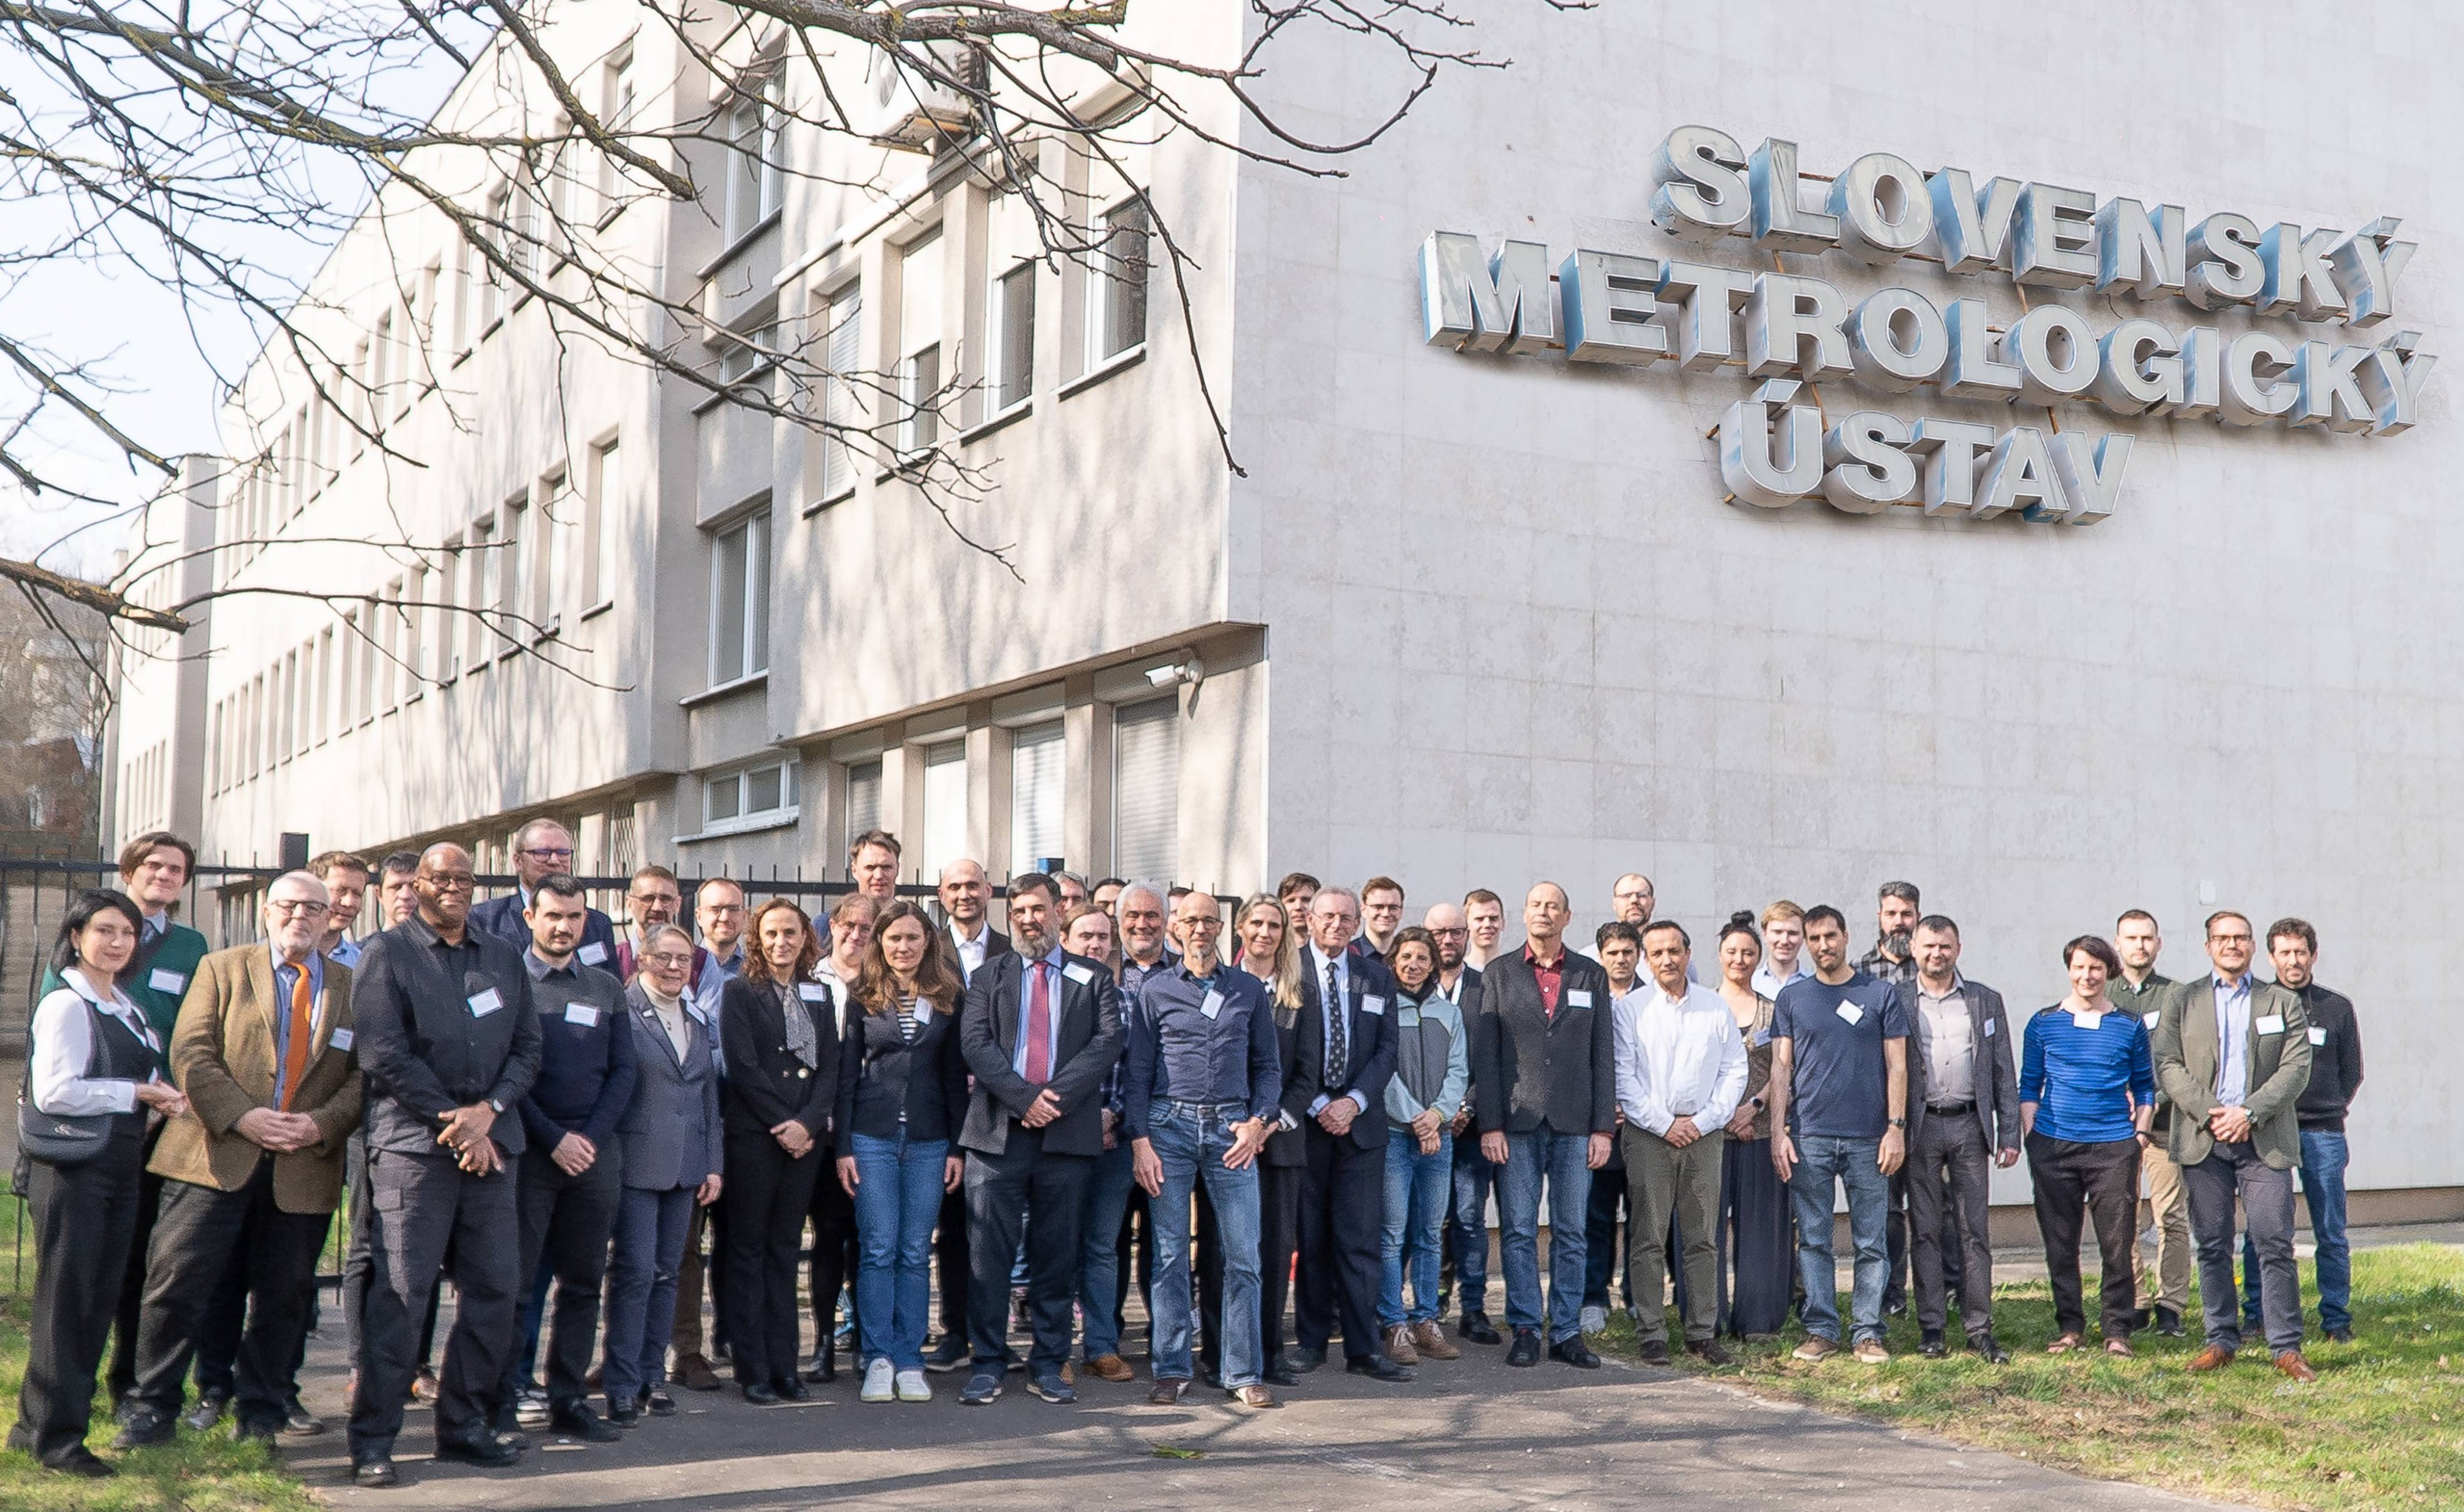
\includegraphics[width=0.9\textwidth, trim=0 0 0 1200, clip]{assets/spring_camp}\\
            \footnotesize
            \textit{25-28 March 2025, Slovak Institute of Metrology, Bratislava, Slovakia}
        \end{center}
    \end{frame}

    \subsection{Topics of interest}

    \begin{frame}
        \frametitle{Topics of interest}
        \begin{columns}%[T,onlytextwidth]
            \begin{column}{0.45\textwidth}
                \begin{block}{Internal}
                    \scriptsize
                    \begin{itemize}
                        \item Activities, interactions, processes, and systems that occur within NMIs or DIs
                        \item Focused on improving the efficiency, accuracy, and reliability of internal operations through digital tools and technologies
                    \end{itemize}
                \end{block}
                \begin{exampleblock}{Deployment}
                    \scriptsize
                    \begin{itemize}
                        \item Implementation and practical application of digital solutions
                        \item It means putting digital tools and technologies into use
                        \item Focused on making digital solutions work effectively in real-world scenarios
                    \end{itemize}
                \end{exampleblock}
            \end{column}
            \begin{column}{0.45\textwidth}
                \begin{block}{External}
                    \scriptsize
                    \begin{itemize}
                        \item Activities and interactions that occur outside NMIs or DIs
                        (customers, industry, other organizations)
                        \item Focused on service delivery, customer experience,
                        and secure and efficient data exchange through digital solutions
                    \end{itemize}
                \end{block}
                \begin{exampleblock}{Research}
                    \scriptsize
                    \begin{itemize}
                        \item Investigation and exploration of new digital technologies and methods
                        \item It means addressing emerging challenges in digitalization
                        \item Focused on discovering and understanding new ways to improve digital processes and systems
                    \end{itemize}
                \end{exampleblock}
            \end{column}
        \end{columns}
    \end{frame}

    \begin{frame}
        \frametitle{Topics of interest}
        \begin{columns}%[T,onlytextwidth]
            \begin{column}{0.45\textwidth}
                \begin{block}{Internal \& deployment}
                    \scriptsize
                    \begin{itemize}
                        \item Internal digital workflows
                        \item Digital tools for comparison analysis
                        \item Using the digital SI framework
                        \item Digital equivalent of traceability
                        \item Remote calibration \& realisation
                    \end{itemize}
                \end{block}
                \begin{block}{External \& deployment}
                    \scriptsize
                    \begin{itemize}
                        \item Smart Digital Calibration Certificates
                        \item QR codes on instruments
                        \item Customer front end
                        \item European common dataspaces
                        \item Digital Quality Infrastructure
                        \item Reference datasets
                        \item Security
                        \item Digital products \& services
                    \end{itemize}
                \end{block}
            \end{column}
            \begin{column}{0.45\textwidth}
                \begin{block}{Internal \& research}
                    \scriptsize
                    \begin{itemize}
                        \item Uncertainties
                        \item Digital workbench
                        \item Blockchain for comparisons
                        \item Research Data Management
                        \item FAIR principles
                        \item Smart calibration guidelines
                    \end{itemize}
                \end{block}
                \begin{block}{External \& research}
                    \scriptsize
                    \begin{itemize}
                        \item Trust in AI
                        \item Machine learning
                        \item Trustworthiness
                        \item Digital twins \& virtual metrology
                        \item Data quality frameworks/principles
                        \item Sensor networks
                        \item Data visualisation (uncertainties)
                    \end{itemize}
                \end{block}
            \end{column}
        \end{columns}
    \end{frame}

    \begin{frame}
        \frametitle{Hot topics of interest}
        \begin{columns}%[T,onlytextwidth]
            \begin{column}{0.45\textwidth}
                \begin{block}{Internal \& deployment}
                    \scriptsize
                    \begin{itemize}
                        \item \highlight{Internal digital workflows}
                        \item \highlight{Digital tools for comparison analysis}
                        \item Using the digital SI framework
                        \item Digital equivalent of traceability
                        \item Remote calibration \& realisation
                    \end{itemize}
                \end{block}
                \begin{block}{External \& deployment}
                    \scriptsize
                    \begin{itemize}
                        \item \highlight{Smart Digital Calibration Certificates}
                        \item QR codes on instruments
                        \item Customer front end
                        \item \highlight{European common dataspaces}
                        \item Digital Quality Infrastructure
                        \item Reference datasets
                        \item Security
                        \item Digital products \& services
                    \end{itemize}
                \end{block}
            \end{column}
            \begin{column}{0.45\textwidth}
                \begin{block}{Internal \& research}
                    \scriptsize
                    \begin{itemize}
                        \item Uncertainties
                        \item Digital workbench
                        \item Blockchain for comparisons
                        \item \highlight{Research Data Management}
                        \item \highlight{FAIR principles}
                        \item Smart calibration guidelines
                    \end{itemize}
                \end{block}
                \begin{block}{External \& research}
                    \scriptsize
                    \begin{itemize}
                        \item Trust in AI
                        \item Machine learning
                        \item \highlight{Trustworthiness}
                        \item Digital twins \& virtual metrology
                        \item \highlight{Data quality frameworks/principles}
                        \item Sensor networks
                        \item Data visualisation (uncertainties)
                    \end{itemize}
                \end{block}
            \end{column}
        \end{columns}
    \end{frame}

    \begin{frame}
        \frametitle{Structured approach to topics of interest}
%        \framesubtitle{Lorem ipsum}
        \begin{columns}[T]
            \column{0.45\textwidth}
            \begin{alertblock}{Core topics}
                \small
                \begin{itemize}

                    \item Software good practice ensuring software quality
                    \item Capacity building
                    \item Policy for data management
                \end{itemize}
            \end{alertblock}
            \column{0.45\textwidth}
            \begin{exampleblock}{Specialized topics}
                \small
                \begin{itemize}
                    \item Vocabulary, metadata and machine readability
                    \item Infrastructure and ecosystem for DCCs
                    \item Framework for advanced analysis
                \end{itemize}
            \end{exampleblock}
        \end{columns}
%        \vspace{1cm} % Adjust the space between the blocks as needed
        \centering
        \begin{minipage}{0.95\textwidth}
            \begin{block}{Facilitator topics}
                \small
                \begin{itemize}
                    \item Sharing and endorsing software
                    \item Knowledge sharing \& Digitalization showcases
                    \item Foster collaborative projects, facilities and workspaces
                    \item Develop links with peer organizations
                \end{itemize}
            \end{block}
        \end{minipage}
    \end{frame}

    \begin{frame}
        \frametitle{Structured approach to topics of interest}
        \framesubtitle{Core topics}
        \begin{itemize}
            \item \textbf{Software good practice \& software quality}
            \begin{itemize}
                \item Develop good practice guides for software development in metrology
                \item Embed software quality as a key element of metrology vía TC-Q
            \end{itemize}
            \item \textbf{Policy for data management}
            \begin{itemize}
                \item Develop example policies for NMIs \& DIs, especially with a view to support smaller NMIs
                \item Create a glossary to inform directors and policy makers
            \end{itemize}
            \item \textbf{Capacity building}
            \begin{itemize}
                \item Provide training for ``casual'' and ``serious'' coders with a metrology focus
                \item Focus on cross-cutting topics including software development and data managment
            \end{itemize}
        \end{itemize}
    \end{frame}

    \begin{frame}
        \frametitle{Structured approach to topics of interest}
        \framesubtitle{Specialized Topics}
        \begin{itemize}
            \item \textbf{Vocabulary, metadata, and machine readability}
            \begin{itemize}
                \item Standardize vocabulary and metadata formats for specific capabilities
                \item Aggregate data to learn about equipment performance and automate/accelerate comparisons
                \item Promote data FAIRness through metadata standardization.
            \end{itemize}
            \item \textbf{Infrastructure and ecosystem for DCCs}
            \begin{itemize}
                \item Define essential components, perform gap analysis, and create roadmaps with TCs and end users
                \item Establish knowledge base, support deployment, provide training for developers and users, disseminate to interest groups
            \end{itemize}
            \item \textbf{Framework for advanced analysis}
            \begin{itemize}
                \item Harmonize testing, trustworthiness, model explainability, data quality assessment, metric and reference data
                \item Improve communication, identify software tools, and create roadmaps with TCs and EMNs
            \end{itemize}
        \end{itemize}
    \end{frame}

    \begin{frame}
        \frametitle{Structured approach to topics of interest}
        \framesubtitle{Facilitator Topics}
        \begin{itemize}
            \item \textbf{Sharing and endorsing software}: Use DCC tools and building blocks as an example to share and peer-review software, accelerating development and building capability
            \item \textbf{Knowledge sharing}: Disseminate collaborative projects outcomes as tools through workshops, and build a knowledge base
            \item \textbf{Digitalization showcases}: Create a library of success stories highlighting the impact of digitalization (save time/money, reduce error, new knowledge)
            \item \textbf{Foster collaboration}: Use an open innovation platform for idea exchange. Facilitate access to examples, software tools and computation facilities
            \item \textbf{Develop links with peer organizations}: BIPM WGs, EMNs, TCs, WELMEC, OIML, JCGM, etc.
        \end{itemize}
    \end{frame}

    \subsection{Common challenges and issues}

    \begin{frame}
        \frametitle{Common challenges and issues}
%        \framesubtitle{Lorem ipsum}
        \begin{itemize}
            \item \textbf{Lack of resources}: Money, computational infrastructure. Communication is key to get them
            \item \textbf{Lack of expert personnel}: Metrologists become programmers, partially or full-time. Workload may also be an issue
            \item \textbf{Lack of common practices and tools}: Each NMI or DI needs a software development/data management strategy.
            A harmonised approach is also needed
            \item \textbf{Lack of shared knowledge and experiences}: Collaboration and communication between NMIs and DIs is key
        \end{itemize}
        \begin{alertblock}{Warning!}
            We are not talking about AI, machine learning or fancy applications.\\
            All of these are related to core or facilitator topics!
        \end{alertblock}
    \end{frame}


    \section{Digitalization for ionizing radiation metrology}

    \begin{frame}
        \frametitle{Digitalization for ionizing radiation metrology}
%        \framesubtitle{Lorem ipsum}
        \centering

        The topics and challenges described before are cross-cutting for al metrology areas
        \bigskip

        \textbf{What are the topics of interest for ionizing radiation metrology?}
        \bigskip

        \textbf{What are your needs and challenges?}
    \end{frame}


    \section{Digitalization activities at CIEMAT}

    \subsection{Needs}

    \begin{frame}
        \frametitle{Digitalization activities at CIEMAT}
%        \framesubtitle{Lorem ipsum}
        \textbf{Laboratory needs}: focused on improving the internal workflow
        \begin{itemize}
            \item \textbf{Digitalization of measurement equipment}: More precise and faster data collection
            \item \textbf{Digitalization of the measurement chain}: Improved data integrity and traceability
            \item \textbf{Automation of data acquisition}: Reduced time and human errors
            \item \textbf{Automation of procedures}: Consistency and precision in processes
        \end{itemize}
        \bigskip

        Dedicated position for digitalization since 2024
    \end{frame}

    \subsection{Digitalization strategy}

    \begin{frame}
        \frametitle{Digitalization strategy at CIEMAT}
        \begin{itemize}
            \item \textbf{Technologies for software development}: Python chosen for its wide adoption in the scientific community and the vast availability of libraries and frameworks that facilitate rapid and efficient development
            \item \textbf{Development philosophy}: Free software, ensures accessibility and modifiability
            \item \textbf{Types of solutions}: Libraries as the foundation for scripts and desktop and web applications
            \item \textbf{Quality assurance}: Documentation, testing, version control, shared development, and continuous integration
            \item \textbf{Code management}: Centralized open organization for easy access and collaboration {\color{blue} \href{https://github.com/lmri-met}{\faExternalLink}}
            \item \textbf{Software distribution}: Via a robust platform widely used by the Python community
        \end{itemize}
    \end{frame}

    \subsection{Digitalization projects}

    \begin{frame}
        \frametitle{Digitalization projects at CIEMAT}
%        \framesubtitle{Lorem ipsum}
        \begin{columns}[T]
            \column{0.45\textwidth}
            \begin{block}{Radionuclide metrology}
                \footnotesize
                \begin{itemize}
                    \item \textbf{MetPyRad library}: Tools for radionuclide metrology: processing measurements an automatic liquid scintillation counter, calculating the half-life of a radionuclide
                    {\color{blue} \href{https://lmri-met.github.io/metpyrad/}{\faExternalLink}}
                    \item \textbf{Desktop application} for data acquisition with a TDCR prototype
                \end{itemize}
            \end{block}

            \column{0.45\textwidth}
            \begin{block}{EURAMET GuideRadPROS Project}
                \footnotesize
                \begin{itemize}
                    \item Project \textbf{website} {\color{blue} \href{https://lmri-met.github.io/sites-guideradpros/}{\faExternalLink}}
                    \item \textbf{USpekPy library}: Uncertainty estimation on protection quantities for x-rays using SpekPy and Monte Carlo techniques
                    {\color{blue} \href{https://github.com/lmri-met/uspekpy}{\faExternalLink}}
                    \item USpekPy \textbf{web application}
                    \item \textbf{Scripts} for x-ray beam characterization
                \end{itemize}
            \end{block}
        \end{columns}
%        \vspace{1cm} % Adjust the space between the blocks as needed
        \centering
        \begin{minipage}{0.95\textwidth}
            \begin{block}{X-ray dosimetry laboratory}
                \footnotesize
                \begin{itemize}
                    \item \textbf{MetPyX library}: Tools for X-ray metrology
                    \item \textbf{Desktop application} for calibration
                \end{itemize}
            \end{block}
        \end{minipage}
    \end{frame}

    \section{}

    \begin{frame}
        \begin{block}{}
            \centering
            Thank you!
        \end{block}
    \end{frame}

\end{document}